% questions.tex —— 2007 年·北京卷·理科 · 题目内容片段（无答案）
% 由 tools/generate_projects.py 依来源总账自 2007/2007_数学真题_北京理_试题.md 生成，勿手改（改源 MD 后重跑）


\gkpart{一、选择题}

\begin{question}
\gkti{1}已知 $\cos\theta\cdot\tan\theta<0$，那么角 $\theta$ 是（　）

（A）第一或第二象限角　（B）第二或第三象限角　（C）第三或第四象限角　（D）第一或第四象限角

\end{question}
\begin{question}
\gkti{2}函数 $f(x)=3^x\ (0<x\leq 2)$ 的反函数的定义域为（　）

（A）$(0,+\infty)$　（B）$(1,9]$　（C）$(0,1)$　（D）$[9,+\infty)$

\end{question}
\begin{question}
\gkti{3}平面 $\alpha\parallel$ 平面 $\beta$ 的一个充分条件是（　）

（A）存在一条直线 $a$，$a\parallel\alpha,\ a\parallel\beta$

（B）存在一条直线 $a$，$a\subset\alpha,\ a\parallel\beta$

（C）存在两条平行直线 $a,b$，$a\subset\alpha,\ b\subset\beta,\ a\parallel\beta,\ b\parallel\alpha$

（D）存在两条异面直线 $a,b$，$a\subset\alpha,\ b\subset\beta,\ a\parallel\beta,\ b\parallel\alpha$

\end{question}
\begin{question}
\gkti{4}已知 $O$ 是 $\triangle ABC$ 所在平面内一点，$D$ 为 $BC$ 边中点，且
$2\overrightarrow{OA}+\overrightarrow{OB}+\overrightarrow{OC}=\vec{0}$，那么（　）

（A）$\overrightarrow{AO}=\overrightarrow{OD}$　（B）$\overrightarrow{AO}=2\overrightarrow{OD}$　（C）$\overrightarrow{AO}=3\overrightarrow{OD}$　（D）$2\overrightarrow{AO}=\overrightarrow{OD}$

\end{question}
\begin{question}
\gkti{5}记者要为 5 名志愿者和他们帮助的 2 位老人拍照，要求排成一排，2 位老人相邻但不排在两端，不同的排法共有（　）

（A）1440 种　（B）960 种　（C）720 种　（D）480 种

\end{question}
\begin{question}
\gkti{6}若不等式组

\nopagebreak[4]
\[
\begin{cases}
x-y\geq 0,\\
2x+y\leq 2,\\
y\geq 0,\\
x+y\leq a,
\end{cases}
\]

表示的平面区域是一个三角形，则 $a$ 的取值范围是（　）

（A）$a\geq\dfrac43$　（B）$0<a\leq 1$　（C）$1\leq a\leq\dfrac43$　（D）$0<a\leq 1$ 或 $a\geq\dfrac43$

\end{question}
\begin{question}
\gkti{7}如果正数 $a,b,c,d$ 满足 $a+b=cd=4$，那么（　）

（A）$ab\leq c+d$，且等号成立时 $a,b,c,d$ 的取值唯一

（B）$ab\geq c+d$，且等号成立时 $a,b,c,d$ 的取值唯一

（C）$ab\leq c+d$，且等号成立时 $a,b,c,d$ 的取值不唯一

（D）$ab\geq c+d$，且等号成立时 $a,b,c,d$ 的取值不唯一

\end{question}
\begin{question}
\gkti{8}对于函数① $f(x)=\lg(|x-2|+1)$，② $f(x)=(x-2)^2$，③ $f(x)=\cos(x+2)$，判断如下三个命题的真假：

命题甲：$f(x+2)$ 是偶函数；

命题乙：$f(x)$ 在 $(-\infty,2)$ 上是减函数，在 $(2,+\infty)$ 上是增函数；

命题丙：$f(x+2)-f(x)$ 在 $(-\infty,+\infty)$ 上是增函数。

能使命题甲、乙、丙均为真的所有函数的序号是（　）

（A）①③　（B）①②　（C）③　（D）②

\end{question}
\gkpart{二、填空题}

\begin{question}
\gkti{9}$\dfrac{2}{(1+i)^2}=$\gkblank{}。

\end{question}
\begin{question}
\gkti{10}若数列 $\{a_n\}$ 的前 $n$ 项和 $S_n=n^2-10n\ (n=1,2,3,\ldots)$，则此数列的通项公式为\gkblank{}；数列 $\{na_n\}$ 中数值最小的项是第\gkblank{}项。

\end{question}
\begin{question}
\gkti{11}在 $\triangle ABC$ 中，若 $\tan A=\dfrac13$，$C=150^\circ$，$BC=1$，则 $AB=$\gkblank{}。

\end{question}
\begin{question}
\gkti{12}已知集合 $A=\{x\mid |x-a|\leq 1\}$，$B=\{x\mid x^2-5x+4\geq 0\}$。若 $A\cap B=\varnothing$，则实数 $a$ 的取值范围是\gkblank{}。

\Needspace{0.4\textheight}
\end{question}
\begin{question}
\gkti{13}2002 年在北京召开的国际数学家大会，会标是以我国古代数学家赵爽的弦图为基础设计的。弦图是由四个全等直角三角形与一个小正方形拼成的一个大正方形（如图）。如果小正方形的面积为 1，大正方形的面积为 25，直角三角形中较小的锐角为 $\theta$，那么 $\cos 2\theta$ 的值等于\gkblank{}。
\nopagebreak[4]
\begin{center}% 依据固定来源 PDF 第 1 页重绘；source_id=src-3612a22ce3848ad6ebbec4d94861dd64b009980e14e8c7a83efefb2ea39bd367
% PDF SHA-256: 2cea664b02860c04aa21fb6bdf80403b674befb8e61fa9f68970197bdf0f5ff4
\begin{center}
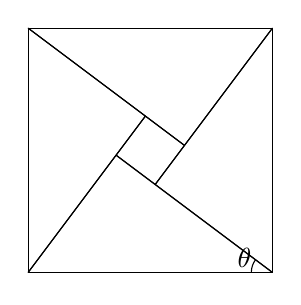
\begin{tikzpicture}[scale=0.62,line join=round,line cap=round]
  \coordinate (A) at (0,0);
  \coordinate (B) at (5,0);
  \coordinate (C) at (5,5);
  \coordinate (D) at (0,5);
  \coordinate (P) at (1.8,2.4);
  \coordinate (Q) at (2.6,1.8);
  \coordinate (R) at (3.2,2.6);
  \coordinate (S) at (2.4,3.2);
  \draw (A)--(B)--(C)--(D)--cycle;
  \draw (A)--(P)--(B);
  \draw (B)--(Q)--(C);
  \draw (C)--(R)--(D);
  \draw (D)--(S)--(A);
  \draw (P)--(Q)--(R)--(S)--cycle;
  \draw (4.57,0) arc[start angle=180,end angle=143.13,radius=0.43];
  \node at (4.43,0.30) {$\theta$};
\end{tikzpicture}
\end{center}
\end{center}
\nopagebreak[4]
\end{question}
\begin{question}
\gkti{14}已知函数 $f(x)$，$g(x)$ 分别由下表给出：

\begin{center}
\begin{tabular}{lrrr}
\toprule
$x$ & 1 & 2 & 3 \\
\midrule
$f(x)$ & 1 & 3 & 1 \\
\bottomrule
\end{tabular}
\end{center}

\begin{center}
\begin{tabular}{lrrr}
\toprule
$x$ & 1 & 2 & 3 \\
\midrule
$g(x)$ & 3 & 2 & 1 \\
\bottomrule
\end{tabular}
\end{center}

则 $f[g(1)]$ 的值为\gkblank{}；满足 $f[g(x)]>g[f(x)]$ 的 $x$ 的值是\gkblank{}。

\end{question}
\gkpart{三、解答题}

\begin{question}
\gkti{15}数列 $\{a_n\}$ 中，$a_1=2,\ a_{n+1}=a_n+cn$（$c$ 是常数，$n=1,2,3,\ldots$），且 $a_1,a_2,a_3$ 成公比不为 1 的等比数列。

（1） 求 $c$ 的值；

（2） 求 $\{a_n\}$ 的通项公式。

\Needspace{0.4\textheight}
\end{question}
\begin{question}
\gkti{16}如图，在 $\mathrm{Rt}\triangle AOB$ 中，$\angle OAB=\dfrac{\pi}{6}$，斜边 $AB=4$。$\mathrm{Rt}\triangle AOC$ 可以通过 $\mathrm{Rt}\triangle AOB$ 以直线 $AO$ 为轴旋转得到，且二面角 $B-AO-C$ 是直二面角。动点 $D$ 在斜边 $AB$ 上。

（1） 求证：平面 $COD\perp$ 平面 $AOB$；

（2） 当 $D$ 为 $AB$ 的中点时，求异面直线 $AO$ 与 $CD$ 所成角的大小；

（3） 求 $CD$ 与平面 $AOB$ 所成角的最大值。
\nopagebreak[4]
\begin{center}% 依据固定来源 PDF 第 1 页的点位、棱线和虚实关系重绘；示意图不按比例
% source_id=src-3612a22ce3848ad6ebbec4d94861dd64b009980e14e8c7a83efefb2ea39bd367
% PDF SHA-256: 2cea664b02860c04aa21fb6bdf80403b674befb8e61fa9f68970197bdf0f5ff4
\begin{center}
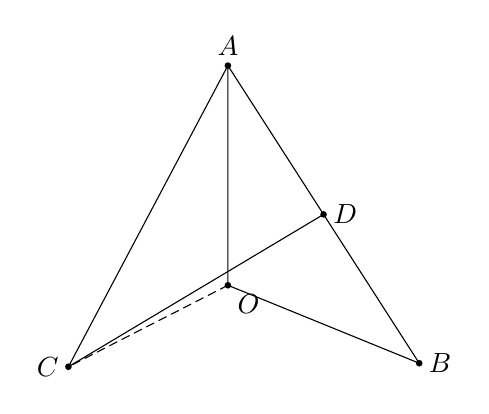
\begin{tikzpicture}[x=0.9cm,y=0.9cm,line join=round,line cap=round]
  \coordinate (A) at (0,3.1);
  \coordinate (O) at (0,0);
  \coordinate (B) at (2.7,-1.1);
  \coordinate (C) at (-2.25,-1.15);
  \coordinate (D) at (1.35,1.0);
  \draw (A)--(B)--(O)--cycle;
  \draw (A)--(C);
  \draw[densely dashed] (O)--(C);
  \draw (C)--(D);
  \fill (A) circle (1.2pt) node[above] {$A$};
  \fill (B) circle (1.2pt) node[right] {$B$};
  \fill (C) circle (1.2pt) node[left] {$C$};
  \fill (O) circle (1.2pt) node[below right] {$O$};
  \fill (D) circle (1.2pt) node[right] {$D$};
\end{tikzpicture}
\end{center}
\end{center}
\nopagebreak[4]
\end{question}
\begin{question}
\gkti{17}矩形 $ABCD$ 的两条对角线相交于点 $M(2,0)$，$AB$ 边所在直线的方程为 $x-3y-6=0$，点 $T(-1,1)$ 在 $AD$ 边所在直线上。

（1） 求 $AD$ 边所在直线的方程；

（2） 求矩形 $ABCD$ 外接圆的方程；

（3） 若动圆 $P$ 过点 $N(-2,0)$，且与矩形 $ABCD$ 的外接圆外切，求动圆 $P$ 的圆心的轨迹方程。

\Needspace{0.4\textheight}
\end{question}
\begin{question}
\gkti{18}某中学号召学生在今年春节期间至少参加一次社会公益活动（以下简称活动），该校合唱团共有 100 名学生，他们参加活动的次数统计如图所示。

图示数据：参加 1 次活动的有 10 人，参加 2 次的有 50 人，参加 3 次的有 40 人；纵轴标“参加人数”，横轴标“活动次数”。

（1） 求合唱团学生参加活动的人均次数；

（2） 从合唱团中任意选两名学生，求他们参加活动次数恰好相等的概率；

（3） 从合唱团中任意选两名学生，用 $\xi$ 表示这两人参加活动次数之差的绝对值，求随机变量 $\xi$ 的分布列及数学期望 $E\xi$。
\nopagebreak[4]
\begin{center}% 依据固定来源 PDF 第 2 页的柱高与坐标轴文字重绘
% source_id=src-3612a22ce3848ad6ebbec4d94861dd64b009980e14e8c7a83efefb2ea39bd367
% PDF SHA-256: 2cea664b02860c04aa21fb6bdf80403b674befb8e61fa9f68970197bdf0f5ff4
\begin{center}
\begin{tikzpicture}[x=0.72cm,y=0.075cm,line join=round]
  \draw[->] (0,0)--(4.7,0) node[right] {活动次数};
  \draw[->] (0,0)--(0,60) node[above] {参加人数};
  \draw (0.65,0) rectangle (1.35,10);
  \draw (1.65,0) rectangle (2.35,50);
  \draw (2.65,0) rectangle (3.35,40);
  \foreach \x/\label in {1/1,2/2,3/3} {
    \draw (\x,0)--(\x,-2.3) node[below] {\label};
  }
  \foreach \y/\label in {10/10,20/20,30/30,40/40,50/50} {
    \draw (-0.08,\y)--(0.08,\y);
    \node[left] at (-0.12,\y) {\label};
  }
\end{tikzpicture}
\end{center}
\end{center}
\nopagebreak[4]
\Needspace{0.4\textheight}
\end{question}
\begin{question}
\gkti{19}如图，有一块半椭圆形钢板，其半轴长为 $2r$，短半轴长为 $r$，计划将此钢板切割成等腰梯形的形状，下底 $AB$ 是半椭圆的短轴，上底 $CD$ 的端点在椭圆上，记 $CD=2x$，梯形面积为 $S$。

（1） 求面积 $S$ 以 $x$ 为自变量的函数式，并写出其定义域；

（2） 求面积 $S$ 的最大值。
\nopagebreak[4]
\begin{center}% 依据固定来源 PDF 第 2 页半椭圆、梯形及两处 2r 尺寸标注重绘
% source_id=src-3612a22ce3848ad6ebbec4d94861dd64b009980e14e8c7a83efefb2ea39bd367
% PDF SHA-256: 2cea664b02860c04aa21fb6bdf80403b674befb8e61fa9f68970197bdf0f5ff4
\begin{center}
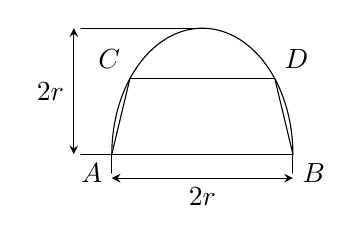
\begin{tikzpicture}[x=1.15cm,y=0.8cm,line join=round,line cap=round,>=stealth]
  \coordinate (A) at (-1,0);
  \coordinate (B) at (1,0);
  \coordinate (C) at (-0.8,1.2);
  \coordinate (D) at (0.8,1.2);
  \draw[domain=180:0,samples=100,smooth,variable=\t] plot ({cos(\t)},{2*sin(\t)});
  \draw (A)--(B);
  \draw (C)--(D);
  \draw (A)--(C);
  \draw (B)--(D);
  \draw[<->] (-1,-0.38)--(1,-0.38) node[midway,below] {$2r$};
  \draw (-1,0)--(-1,-0.30);
  \draw (1,0)--(1,-0.30);
  \draw[<->] (-1.42,0)--(-1.42,2) node[midway,left] {$2r$};
  \draw (-1,0)--(-1.34,0);
  \draw (0,2)--(-1.34,2);
  \node[below left] at (A) {$A$};
  \node[below right] at (B) {$B$};
  \node[above left] at (C) {$C$};
  \node[above right] at (D) {$D$};
\end{tikzpicture}
\end{center}
\end{center}
\nopagebreak[4]
\begin{gktip}

\textbf{原文疑点（ISSUE-1203，未决）}：题干印作“其半轴长为 $2r$，短半轴长为 $r$”；保留原文，未擅自补成“长半轴长”。
\end{gktip}

\end{question}
\begin{question}
\gkti{20}已知集合 $A=\{a_1,a_2,\ldots,a_k\}\ (k\geq 2)$，其中 $a_i\in\mathbb{Z}\ (i=1,2,\ldots,k)$。由 $A$ 中的元素构成两个相应的集合：

\nopagebreak[4]
\[
S=\{(a,b)\mid a\in A,\ b\in A,\ a+b\in A\};\qquad
T=\{(a,b)\mid a\in A,\ b\in A,\ a-b\in A\},
\]

其中 $(a,b)$ 是有序数对，集合 $S$ 和 $T$ 中的元素个数分别为 $m$ 和 $n$。若对于任意的 $a\in A$，总有 $-a\notin A$，则称集合 $A$ 具有性质 $P$。

（1） 检验集合 $\{0,1,2,3\}$ 与 $\{-1,2,3\}$ 是否具有性质 $P$，并对其中具有性质 $P$ 的集合，写出相应的集合 $S$ 和 $T$；

（2） 对任何具有性质 $P$ 的集合 $A$，证明：$n\leq \dfrac{k(k-1)}2$；

（3） 判断 $m$ 和 $n$ 的大小关系，并证明你的结论。

\begin{gktip}
\textbf{来源说明}：本题面逐题依据固定来源 PDF（2 页 A3，印刷页码 351–352）转录，source ID 为 \texttt{src-3612a22ce3848ad6ebbec4d94861dd64b009980e14e8c7a83efefb2ea39bd367}，SHA-256 为 \texttt{2cea664b02860c04aa21fb6bdf80403b674befb8e61fa9f68970197bdf0f5ff4}。固定源没有答案、解析或评分标准；发布者、出版信息、版本及官方身份未核。图形尚待矢量重绘。题19“半轴长”按原文保留，术语含义待核。
\end{gktip}

\end{question}